\documentclass[14pt]{beamer}
\usepackage{beamerthemeshadow}
\usepackage{graphicx}
\usepackage{color}
\usepackage[utf8]{inputenc}
\usepackage{hyperref}
\usepackage{makecell}                       %potrebno za formatiranje tabele
%\usepackage[flushleft]{threeparttable}     %ne koristimo ovo?

\usepackage[english, serbian]{babel}        %da ne bi pisalo "Table" nego "Tabela" i slično

\definecolor{electricpurple}{rgb}{0.75, 0.0, 1.0}
\setbeamercolor{structure}{fg=electricpurple}

\def\d{{\fontencoding{T1}\selectfont\dj}}
\def\D{{\fontencoding{T1}\selectfont\DJ}}


\title{Analogni računari}
\subtitle{-- Tehničko i naučno pisanje --}
\author{Aleksandar Končalović, Veljko Josipović, Veljko Strugar, Uroš Janković}
\institute{Matematički fakultet\\Univerzitet u Beogradu}
\date{
	\footnotesize{Beograd, 2022.}	
}

\begin{document}
\begin{frame}
	\thispagestyle{empty}
	\titlepage
\end{frame}

\addtocounter{framenumber}{-1}

\section{Princip rada}

\begin{frame}[fragile]\frametitle{Princip rada analognih računara}
	\begin{itemize}	
		\item Obrađivanje kontinualnih veličina
		  \begin{itemize}
                \item Količina vode u cevima, intenzitet magnetne sile, vibracije tla kod seizmografa temperatura raznih supstanci...
            \end{itemize}          
	

\item Operacija sabiranja dva broja

\item Operacija množenja dva broja \\ $$ U = R*I $$
\end{itemize}
\begin{figure}[h!]
\begin{center}
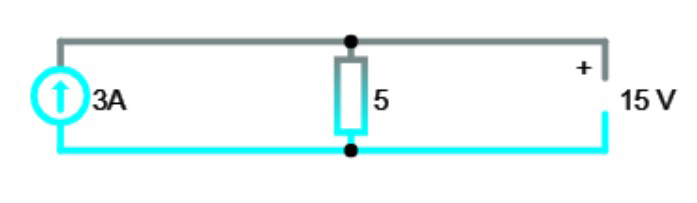
\includegraphics[scale=0.6]{Struja.jpg}
\end{center}
\caption{Vizuelni prikaz množenja}
\label{fig:h1}
\end{figure}
\end{frame}

\section{Hidrointregrator Mike Alasa}
\begin{frame}{Hidrointegrator Mike Alasa}
\begin{itemize}
    \item Najavio Ljubomir Klerić 1896.
    \item Završen 1899.
\end{itemize}
\begin{figure}[h!]
\begin{center}
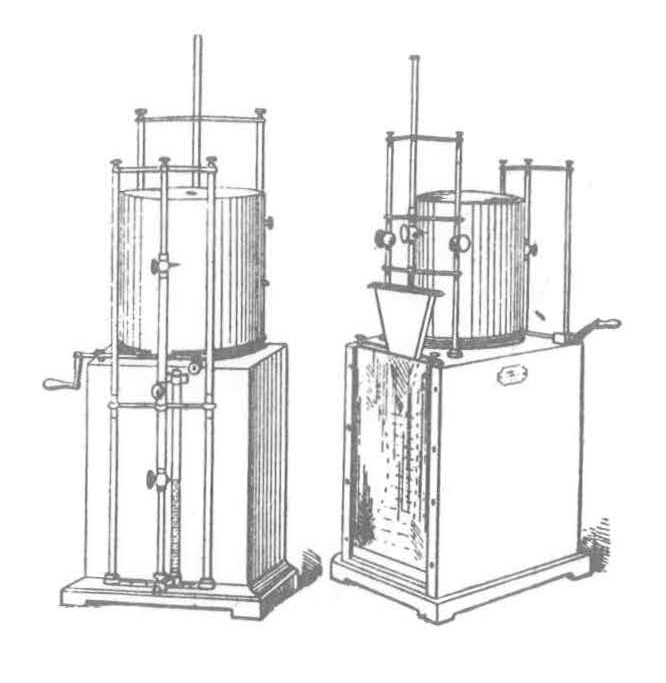
\includegraphics[scale=0.6]{h1.jpg}
\end{center}
\caption{Petrovićeva skica hidrointegratora. }
\label{fig:h1}
\end{figure}
    
\end{frame}


\section{Literatura}

\begin{frame}[fragile]\frametitle{Literatura}
	\begin{itemize}	
		\scriptsize \item Jo Marchant, "Archimedes and the 2000-year-old computer" New Scientist, 12 December 2008.

\scriptsize \item E G Fischer (1912), "The Coast and Geodetic Survey Tide Predicting Machine No. 2".

\scriptsize \item Srpska akademija nauka i umetnosti, "Hidrointegrator Mihaila Petrovića Alasa". Pristupljeno 6.11.2022.

\scriptsize \item Thomas H. Lange. "Peenemuende, Analyse einer Technologieentwicklung im Dritten Reich". VDI-Verlag, Dusseldorf, 2006.
			
\scriptsize \item Bissell, C.C. (2004). "A great disappearing act: the electronic analogue computer". IEEE Conference on the History of Electronics, Bletchley, UK, 28-30 Jun 2004.
\end{itemize}
\end{frame}

\end{document}